\chapter{Experiment results}

%\textbf{Insert time and perpelexity here.}

\section{Baseline model}

\subsection{Acoustic model AM.200 and Language Model Version 1 (LM.200.1e-9)}
\label{amv0s1}


Calculating PMER and WMER for each segment by utilizing AM.200 and LM.200.1e-9:
\begin{enumerate}
\item GMM(GMM.200): GMM is trained by using the 200 hours data
\item TDNN(TDNN.200): the result of GMM training(GMM.200) is utilized to build a TDNN(time delay neural network). 
\item TDNN graph creation \\
The language model used is the LM.200.1e-9 and  the acoustic model is  TDNN.200; furthermore, the dictionary used(Lexicon.200) is the modification of the library provided by MGB(Lexicon.MGB). Words in Lexicon.MGB which do not exist in word.200 are removed from Lexicon.200.
%\item TDNN development set recognition \\
%The development set is files from dev.short, which contains 8 hours of audio. The development set is recognized by leveraging the graph created in the previous step.
\item TDNN 200 hours of training data recognition \\
We need to recognize 200 hours data to calculate PMER, WMER, and AWD. This data will be used for data selection of the next iteration.
\item Sclite score PMER and WMER \\
Use the lattice and graph(produced at step 5 and 3 respectively) to calculate overall PMER and WMER. However, the decoding program does not provide PMER, WMER, and AWD for each segment. Fortunately, the program generates prf file which contains number of correction, insertion, deletion, and substitution for each segment. Two prf files exist after decoding:(ctm\_words.filt.filt.prf contains word match error rate and ctm\_phones.filt.filt.prf contains phone match error rate). From there, we are able to calculate  PMER, WMER, and AWD of each segments.  For the development set, we only need to know the overall PER and WER. In contrast, training set recognition needs PMER, WMER, and AWD for each segment. 

\end{enumerate}


version AM0
% table
\begin{center}
\begin{tabular}{ | c | c | c | c |  c |  }
\hline
\textbf{No.} & \textbf{Description} & \textbf{Result} & \textbf{execution time} & \textbf{extra info} \\ \hline \hline
1 & GMM.100  &  & 3h 30m & 20 hosts \\  \hline
%/talc2/multispeech/calcul/users/jkarsten/mgb/recipe/tools/baseline/baseline1_backup/gmm
%1.1 & GMM decoding & 57.2\% WER  & 3h 36m 47s & 20 hosts, 4 cores \\  \hline \hline
%2 & AM.200 training. &  & 38h 30m 31s & 3 nodes \\  

2 & TDNN.100 training: & & 17h 7m & 3 GPU hosts \\ 
 & LM.200.1e-9,  GMM.100, Lexicon.200 &  & & \\ \hline
 %/talc2/multispeech/calcul/users/jkarsten/mgb/recipe/tools/baseline/baseline1_backup/tdnn
 
3 & Create a graph from TDNN.200,  &  & 6m & 1 host \\  
 & LM.200.1e-9, Lexicon.200  & & & \\ \hline
%/talc2/multispeech/calcul/users/jkarsten/mgb/recipe/tools/modifASR/tdnn_s1/graph_creation_from_arpaLM

4 & Create a graph from TDNN.200,  &   & 4h 49m & 1 host \\  
 & LM.7weeks+subtitles.1e-9, Lexicon.200  & & & \\ \hline

%4 & AM.200 recognized dev.short &  & 2h 58m 58s   & 20 hosts  \\  \hline
5 & TDNN.100 recognized train.200 &  & 16h 6m & 20 hosts \\  \hline 
 %/talc2/multispeech/calcul/users/jkarsten/mgb/recipe/tools/modifASR/tdnn_s1/recognition_with_scoring/decode_res_train_200_fst+merall_mgb2015.wordList.4gm.kn.arpa.gz.1e-9.arpa_4thr

6 & TDNN.100 \& LM.7weeks+subtitles.1e-9 & WER 43.9\%   & 45m & 20 hosts \\  
&  recognized dev.short & PER 35.8\% & & \\ \hline
%5 & Calculate Overall PMER & 24.8 \% PMER   & 5h 5m 51s & 1 host \\  \
 %& and WMER of train.200  & 32.4 \% WMER & & \\ \hline
%5.1 &  Calculate PMER and WMER & & 20m 22s & 1 host \\  
 %&  per segment of step 6 & & &  \\  \hline
%/talc2/multispeech/calcul/users/jkarsten/mgb/recipe/tools/modifASR/tdnn_s1/sclite_score_pmer_and_wmer
% /talc2/multispeech/calcul/users/jkarsten/mgb/recipe/tools/modifASR/tdnn_s1/calculate_pmer_wmer_per_segments

%6 & Calculate PER  &  32.5 \% PER  & 1h 10m 57s   & 1 host \\  \
% & PMER, WMER calculation  &   48.7\% WER   & & \\ \hline
\end{tabular}
\end{center}


%%%%%%%%%%%%%%%%%%%%%%%%%%%%%%%%%%%%%%%%
% table
version AM1
\begin{center}
\begin{tabular}{ | c | c | c | c |  c |  }
\hline
\textbf{No.} & \textbf{Description} & \textbf{Result} & \textbf{execution time} & \textbf{extra info} \\ \hline \hline
1 & GMM.100  &  & 4h 7m & 20 hosts \\  \hline

2 & TDNN.100 training: & & 20h 1m & 3 GPU hosts \\ 
 & LM.200.1e-9,  GMM.100, Lexicon.200 &  & & \\ \hline
 
3 & Create a graph from TDNN.200,  &  & 5m & 1 host \\  
 & LM.200.1e-9, Lexicon.200  & & & \\ \hline
 
4 & Create a graph from TDNN.200,  &   & 3h 7m & 1 host \\  
 & LM.7weeks+subtitles.1e-9, Lexicon.200  & & & \\ \hline

5 & TDNN.100 recognized train.200 &  & 14h 18m & 20 hosts \\  \hline 

6 & TDNN.100 \& LM.7weeks+subtitles.1e-9 & WER 41.2\%   & 46m & 20 hosts \\  
&  recognized dev.short & PER 33.8\% & & \\ \hline
\end{tabular}
\end{center}

%%%%%%%%%%%%%%%%%%%%%%%%%%%%%%%%%%%%%%%%
version AM2
\begin{center}
\begin{tabular}{ | c | c | c | c |  c |  }
\hline
\textbf{No.} & \textbf{Description} & \textbf{Result} & \textbf{execution time} & \textbf{extra info} \\ \hline \hline
1 & GMM.100  &  & 3h 3m & 20 hosts \\  \hline

2 & TDNN.100 training: & & 23h 58m & 3 GPU hosts \\ 
 & LM.200.1e-9,  GMM.100, Lexicon.200 &  & & \\ \hline
 
3 & Create a graph from TDNN.200,  &  & 5m & 1 host \\  
 & LM.200.1e-9, Lexicon.200  & & & \\ \hline
 
4 & Create a graph from TDNN.200,  &   & 3h 13m & 1 host \\  
 & LM.7weeks+subtitles.1e-9, Lexicon.200  & & & \\ \hline

5 & TDNN.100 recognized train.200 &  & 15h 51m & 20 hosts \\  \hline 

6 & TDNN.100 \& LM.7weeks+subtitles.1e-9 & WER 40.5\%   & 36m & 20 hosts \\  
&  recognized dev.short & PER 33.3\% & & \\ \hline
\end{tabular}
\end{center}


%%%%%%%%%%%%%%%%%%%%%%%%%%%%%%%%%%%%%%%%
version AM2
\begin{center}
\begin{tabular}{ | c | c | c | c |  c |  }
\hline
\textbf{No.} & \textbf{Description} & \textbf{Result} & \textbf{execution time} & \textbf{extra info} \\ \hline \hline
1 & GMM.100  &  & 3h 3m & 20 hosts \\  \hline

2 & TDNN.100 training: & & 25h 27m & 3 GPU hosts \\ 
 & LM.200.1e-9,  GMM.100, Lexicon.200 &  & & \\ \hline
 
3 & Create a graph from TDNN.200,  &  & 7m & 1 host \\  
 & LM.200.1e-9, Lexicon.200  & & & \\ \hline
 
4 & Create a graph from TDNN.200,  &   & 4h 49m & 1 host \\  
 & LM.7weeks+subtitles.1e-9, Lexicon.200  & & & \\ \hline

5 & Create a graph from TDNN.200,  &   & 2h 1m each genre & 1 host \\  
 & LM.genres.1e-9, Lexicon.200  & & & \\ \hline

6 & TDNN.100 recognized train.200 &  & 15h 52m & 20 hosts \\  \hline 

7 & TDNN.100 \& LM.7weeks+subtitles.1e-9 & WER 40.5\%   & 38m & 20 hosts \\  
&  recognized dev.short & PER 33.3\% & & \\ \hline
\end{tabular}
\end{center}



%\subsection{Acoustic model AM.200 and Language Model LM.7weeks+subtitles.limited.1e-9}
% table
%\begin{center}
%\begin{tabular}{ | c | c | c | c |  c |  }
%\hline
%\textbf{No.} & \textbf{Description} & \textbf{Result} & \textbf{execution time} & \textbf{extra info} \\ \hline \hline
%3 & Create a graph from TDNN.200,  &  & 3h 12m 25s & 1 host \\   
% & LM.7weeks+subtitles.limited.1e-9,   & & & \\ 
% & Lexicon.7weeks+subtitles & & & \\ \hline
 %/talc2/multispeech/calcul/users/jkarsten/mgb/recipe/tools/modifASR/tdnn_s2/graph_creation_from_arpaLM


%4 & TDNN.200 &  & 1h 10m 59s & 20 hosts \\  
% & recognized dev.short & & & \\ \hline
% /talc2/multispeech/calcul/users/jkarsten/mgb/recipe/tools/modifASR/tdnn_s2/recognition_human/recognition_with_scoring_human


 %5 & TDNN.200 recognized &  & 10h 9m 35s & 20 hosts \\  
 %& train.200 & & & \\ \hline  
 %/talc2/multispeech/calcul/users/jkarsten/mgb/recipe/tools/modifASR/tdnn_s2/recognition_with_scoring
 
% 6 & TDNN AM.200 dev short & 31.8\% PER  & 4h 58m 26s & 1 hosts \\  
% & PMER, WMER calculation & 49.5\% WER & & \\ \hline
% 6.1 & TDNN AM-V0 train 200 & 26.4\% PMER & 4h 58m 26s & 1 hosts \\  
% & PMER, WMER calculation & 39.7\% WMER  & & \\ \hline
% 6.2 & Calculate PMER, WMER &  &  & 1 hosts \\  
 %& AWD per segment &  & & \\ \hline \hline
%\end{tabular}
%\end{center}


\subsection{Acoustic model(AM.200) and Language Model version 3(LM.genres)}


\subsection{Acoustic model AM.100-v1 and Language Model version 1 (LM.200.1e-9)}
% table
\subsubsection{100 hours selection(100-v1)}
How to select 100 hours subset of data for baseline model v1:
Section \ref{amv0s1}  calculates PMER, WMER, and AWD for each segments. Consequently, we can extract segments(of 200 hours transcriptions) which satisfy $0.165 \le AWD \le 0.66$. In the other word, the segments which does not satisfy are removed. Then, segments are sorted based on their PMER in ascending. We can deduce PMER threshold  and its total duration by sorting PMER as presented in the following table:  
\begin{center}
\label{pmerAM0s1}
\begin{tabular}{ | c | c | c | }
\hline
\textbf{PMER} & \textbf{Total duration} & \textbf{Percentage of total segment duration}  \\ \hline \hline
0.0 & 14.83 h & 10\% \\ \hline
5 & 29.66 h & 20\% \\ \hline
10 & 44.49 h & 30\% \\ \hline
16 & 59.32 h & 40\% \\ \hline
24 &  74.15 h & 50\% \\ \hline
33 & 88.98 h & 60\% \\ \hline
47 & 103.81 h & 70\% \\ \hline
82 & 118.64 h & 80\% \\ \hline
\end{tabular}
\end{center}


%PMER: 0.0; duration: 53389.43; percentage: 0.100003435255
%PMER: 0.05; duration: 106776.9; percentage: 0.200003199245
%PMER: 0.1; duration: 160166.65; percentage: 0.30000723389
%PMER: 0.16; duration: 213552.14; percentage: 0.400003289154
%PMER: 0.24; duration: 266939.76; percentage: 0.500003334108
%PMER: 0.33; duration: 320342.37; percentage: 0.600031456745
%PMER: 0.47; duration: 373713.84; percentage: 0.700001251227
%PMER: 0.82; duration: 427112.53; percentage: 0.800022031335

The Table \ref{pmerAM0s1} shows that 60\% of data has 33\% PMER with total duration of 88.98 hours of audio. From the table, we conclude that threshold 33 is selected as the threshold to select data for the next iteration.

\begin{center}
\label{wmerAM0s1}
\begin{tabular}{ | c | c | c | }
\hline
\textbf{WMER} & \textbf{Total duration} & \textbf{Percentage of total segment duration}  \\ \hline \hline
0.0 & 14.83 h & 10\% \\ \hline
8 & 29.66 h & 20\% \\ \hline
15 & 44.49 h & 30\% \\ \hline
23 & 59.32 h & 40\% \\ \hline
32 &  74.15 h & 50\% \\ \hline
43 & 88.98 h & 60\% \\ \hline
58 & 103.81 h & 70\% \\ \hline
98 & 118.64 h & 80\% \\ \hline
\end{tabular}
\end{center}

\subsubsection{Training Acoustic model AM.100-v1}



%\begin{center}
%\begin{tabular}{ | c | c | c | c |  c |  }
%\hline
%\textbf{No.} & \textbf{Description} & \textbf{Result} & \textbf{execution time} & \textbf{extra info} \\ \hline \hline
%1 & GMM.100-v1 &  & 3h 28m 43s & 20 hosts \\  \hline
%2 & TDNN.100-v1 &  & 26h 5m 3s & 3 hosts \\  \hline
%3 & GMM.100-v1\_decode &  & 2h 51m 4s & 20 hosts \\  \hline
%4 & TDNN.100-v1\_decode &  & 24h 30m 31s & 3 hosts \\  \hline
%\end{tabular}
%\end{center}


\subsection{The Second Acoustic model(AM.100-v2) and Language Model version 1 (LM.200.1e-9)}


%\begin{figure}
%\caption{Graph of PMER and WMER produced transcription AM-V0 and LM s1. The red line represents PMER, while the blue line represents WMER.}
%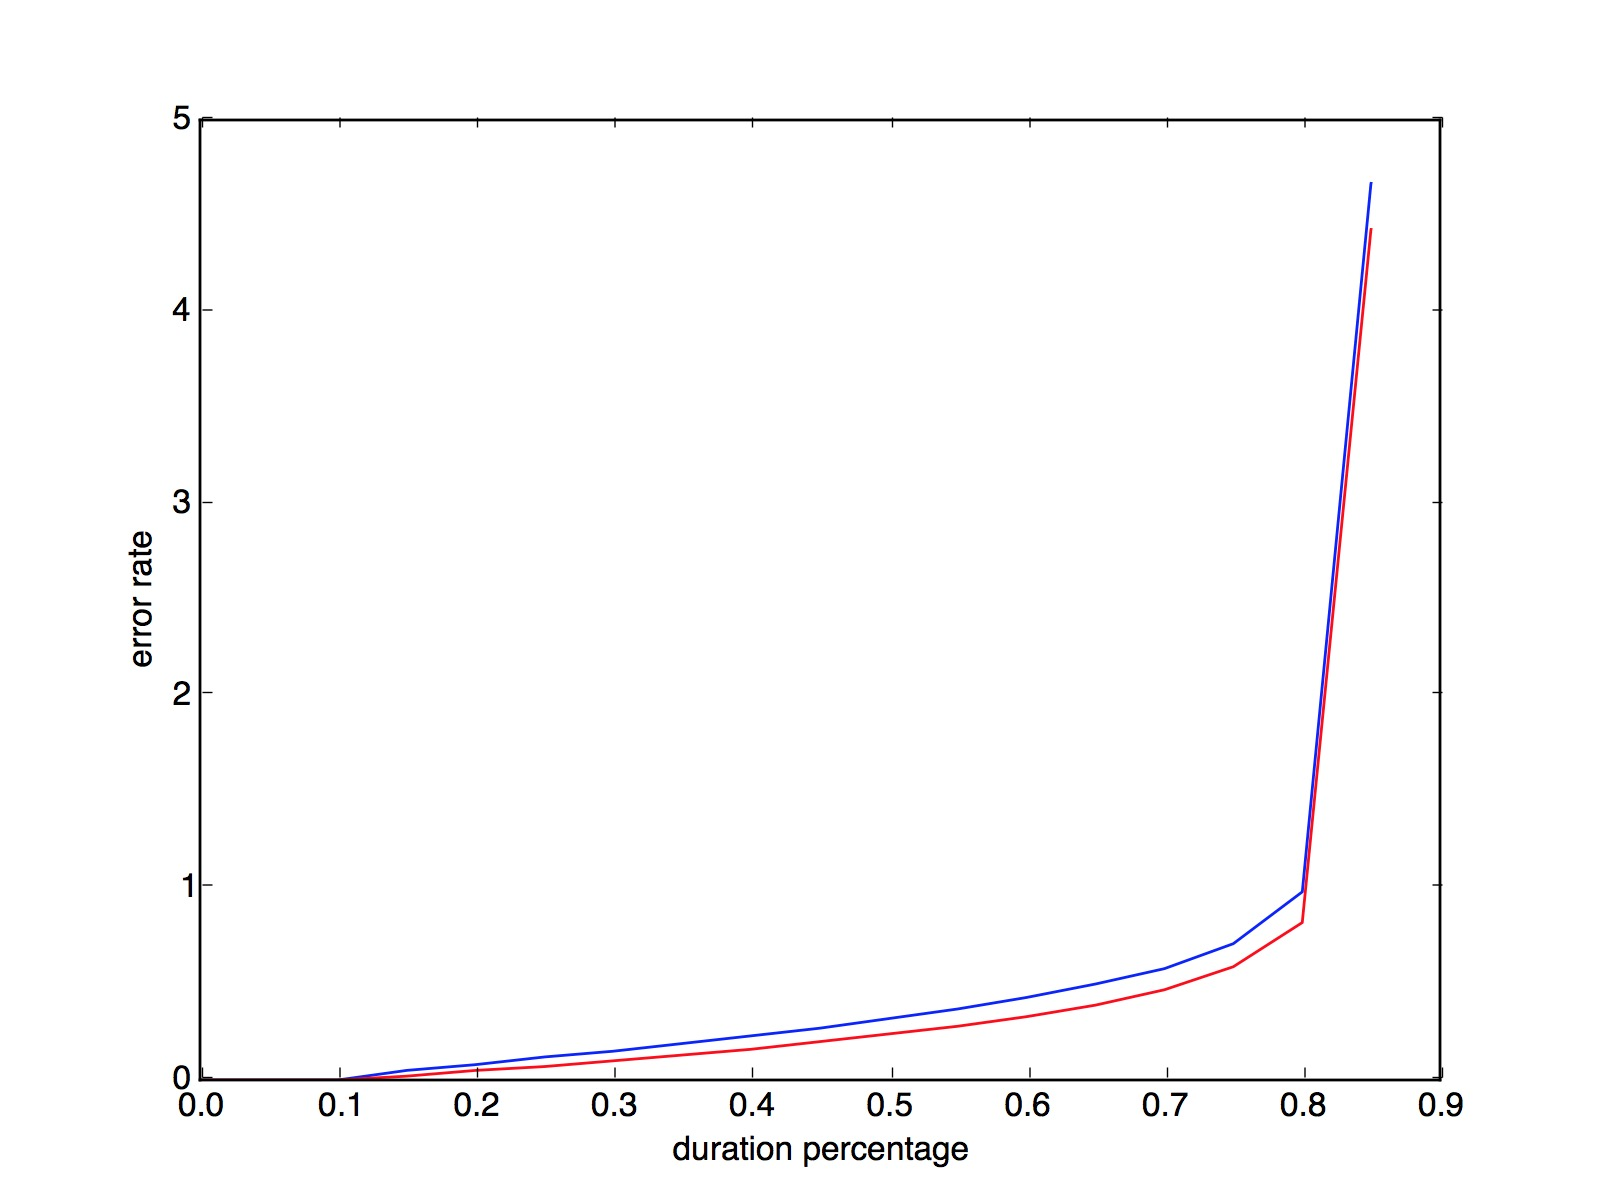
\includegraphics[scale=0.2]{wmerpmeram0s1} 
%\centering
%\end{figure}

%\begin{figure}
%\caption{Graph of PMER and WMER from transcription align, provided by MGB.}
%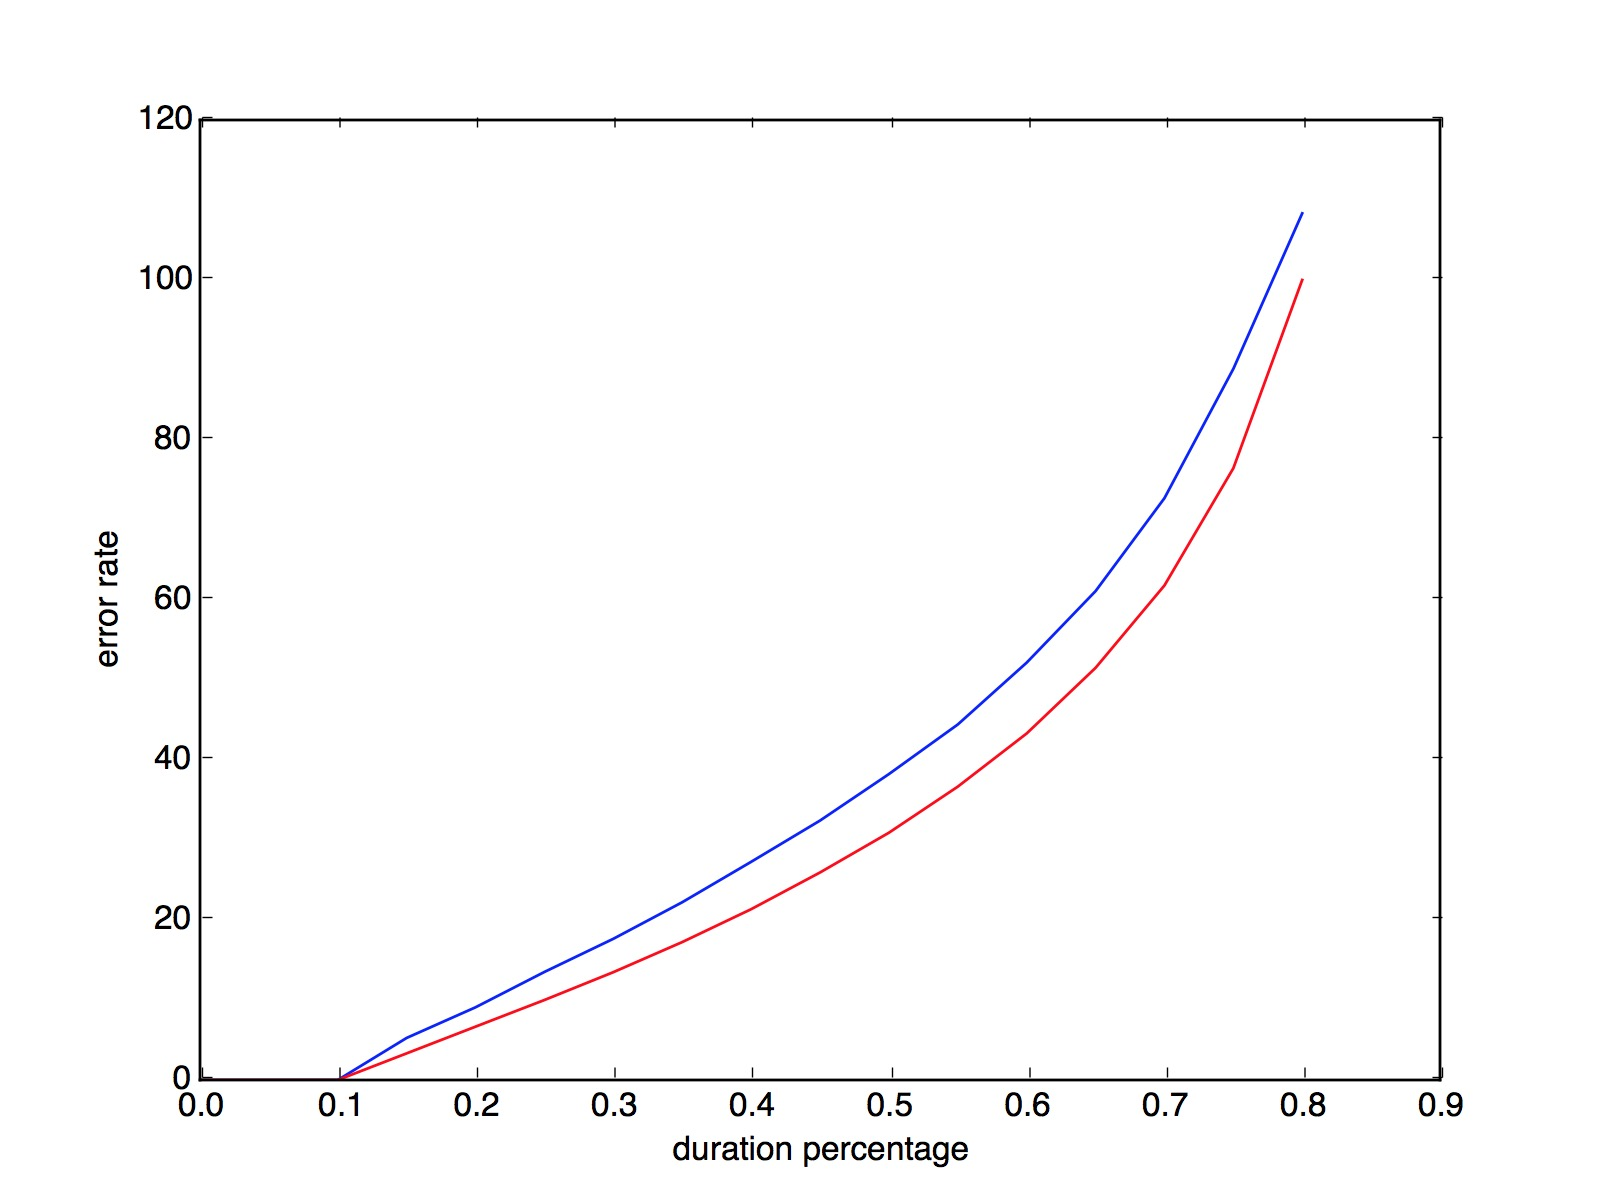
\includegraphics[scale=0.2]{wmerpmeram0align}
%\centering
%\end{figure}

%\subsubsection{Training acoustic model AM.100-v2}
%\begin{center}
%\begin{tabular}{ | c | c | c | c |  c |  }
%\hline
%\textbf{No.} & \textbf{Description} & \textbf{Result} & \textbf{execution time} & \textbf{extra info} \\ \hline \hline
%1 & GMM-V2\_decode &  & 2h 56m 41s & 20 hosts \\  \hline
%2 & TDNN-V2\_decode &  & 23h 52m 58s & 3 hosts \\  \hline
%\end{tabular}
%\end{center}


\section{Comparison}

Comparison between different speech recognizer:
\begin{center}
\label{wmerAM0s1}
\begin{tabular}{ | c | c | c |  c | c |  }
\hline
\textbf{No.} & \textbf{Acoustic model} & \textbf{Language Model}  &  \textbf{PER}  & \textbf{WER}  \\ \hline \hline
1 & TDNN.100  & LM.7weeks+subtitles.limited.1e-9 & 35.8  & 43.9 \\ 
& & Lexicon.7weeks+subtitles  & & \\ \hline


2 & TDNN.100-v1\_decode   & LM.7weeks+subtitles.limited.1e-9  & 34.3    & 42.3 \\
&  & Lexicon.7weeks+subtitles & & \\ \hline

3 & TDNN.100-v1   & LM.7weeks+subtitles.limited.1e-9  & 33.8   & 41.2 \\
&  & Lexicon.7weeks+subtitles & & \\ \hline


4 & TDNN.100-v2   & LM.7weeks+subtitles.limited.1e-9  & 33.3    & 40.5 \\
&  & Lexicon.7weeks+subtitles & & \\ \hline

5 & TDNN.100-v3   & LM.7weeks+subtitles.limited.1e-9  & 33.3    & 40.5 \\
&  & Lexicon.7weeks+subtitles & & \\ \hline
\end{tabular}
\end{center}


\begin{figure}
\caption{Average word duration}
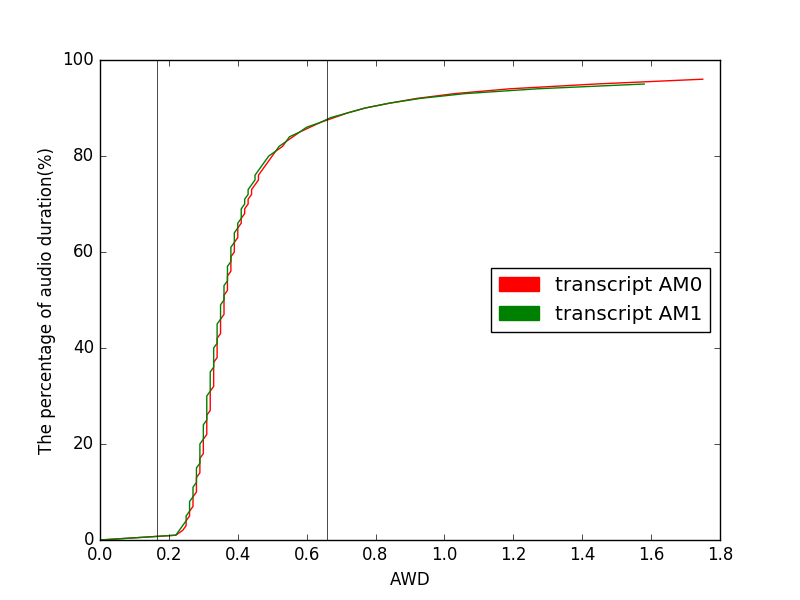
\includegraphics[scale=0.7]{awdLineChart}
\centering
\end{figure}

\begin{figure}
\caption{Phone match error rate}
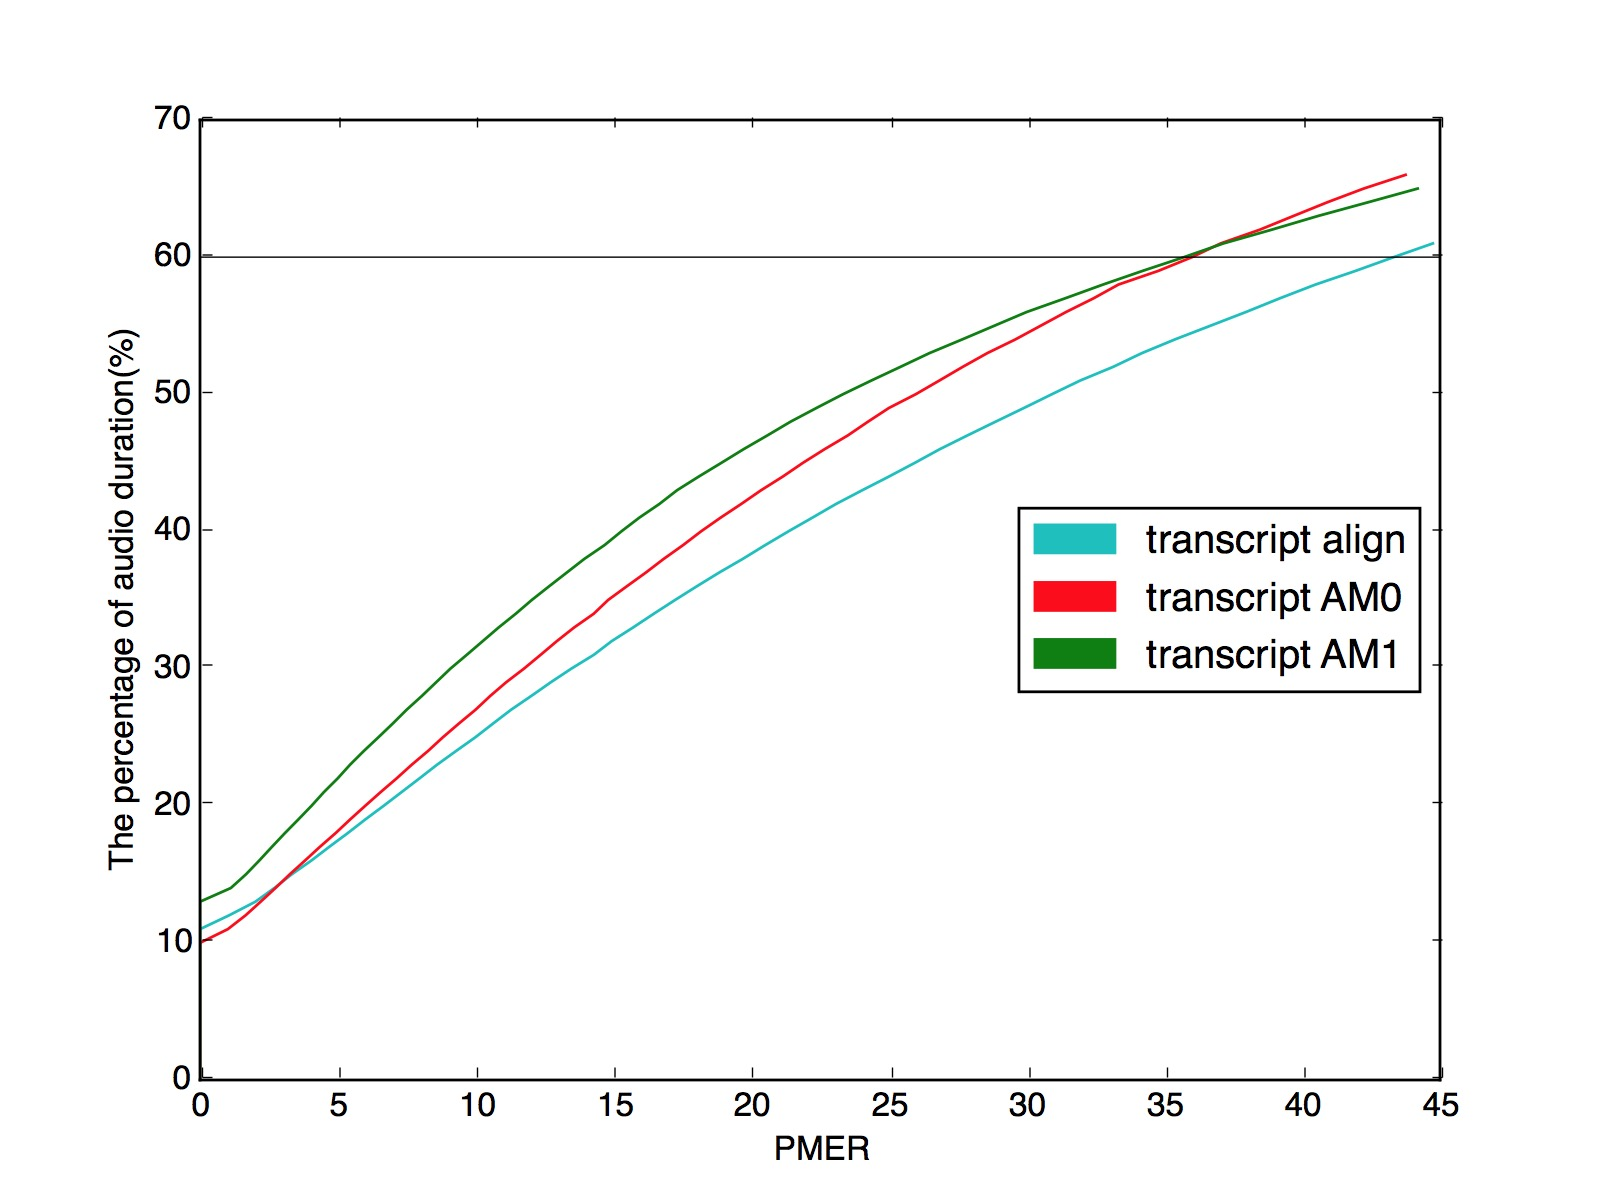
\includegraphics[scale=0.3]{pmerLineChart}
\centering
\end{figure}

\begin{figure}
\caption{Word match error rate}
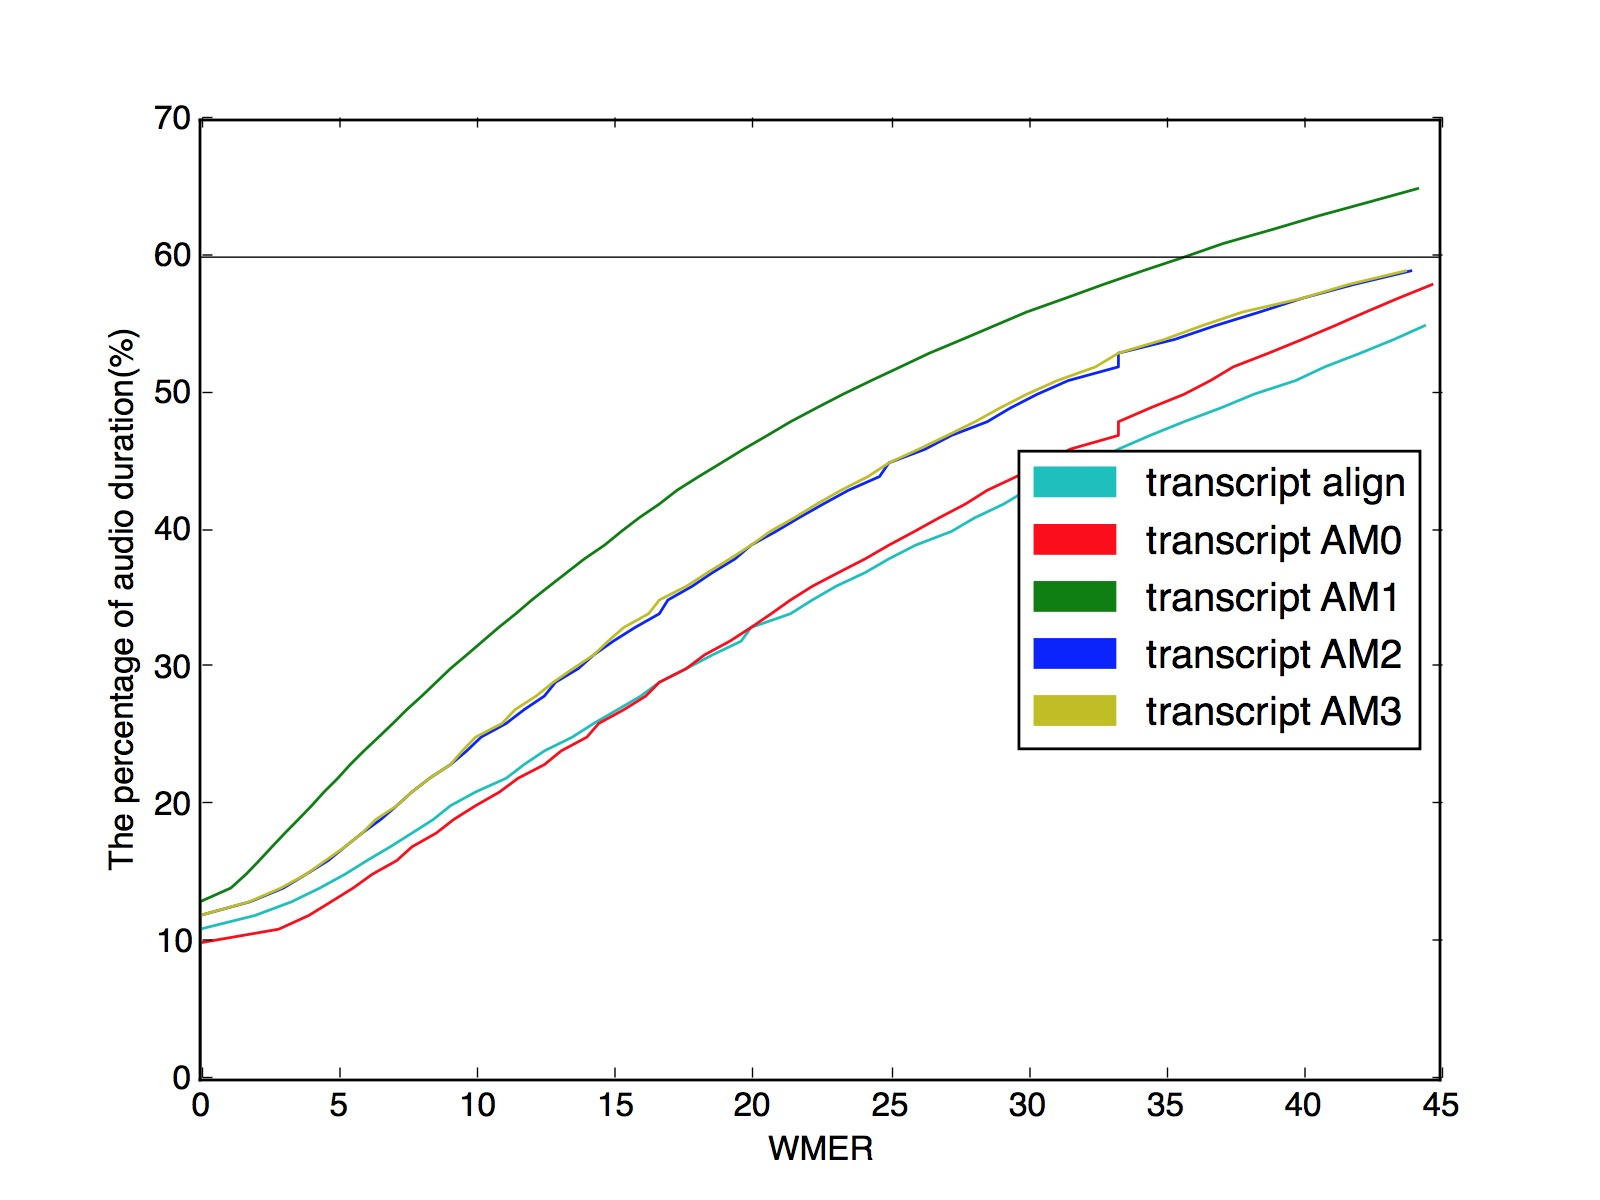
\includegraphics[scale=0.25]{wmerLineChart}
\centering
\end{figure}




%PER 32.2 | 9118 204786 | 75.0 10.0 15.0 7.2 32.2 82.7 | -1.058 | |
%WER 49.3 | 9118 64248 | 59.0 25.1 15.9 8.2 49.3 83.7 | -0.822 | |

%AM0_s1
%WMER
%[0, 0.05001182297101408, 0.1000055705823501, 0.15002999947778156, 0.20000377990423135, 0.250006911717846, 0.3000083202847346, 0.350008061797726, 0.4000080655439148, 0.45000218777410367, 0.5000070802963298, 0.5500076834326855, 0.6000113209817511, 0.6500022214898035, 0.7000031243212423, 0.7500004870045146, 0.8000498093227562, 0.8500152732106541]
%[0, 0.0, 0.0, 0.05, 0.08, 0.12, 0.15, 0.19, 0.23, 0.27, 0.32, 0.37, 0.43, 0.5, 0.58, 0.71, 0.98, 4.67]

%PMER
%[0, 0.05000255115439209, 0.10000343525488571, 0.15000458158857732, 0.20000319924500873, 0.2500218028172682, 0.3000072338900607, 0.3500012437345947, 0.4000032891535333, 0.45000364878763255, 0.5000033341077957, 0.5500060913025576, 0.6000314567451253, 0.6500026335705453, 0.700001251226977, 0.7500149847541436, 0.8000220313347739, 0.8500007005372576]
%[0, 0.0, 0.0, 0.02, 0.05, 0.07, 0.1, 0.13, 0.16, 0.2, 0.24, 0.28, 0.33, 0.39, 0.47, 0.59, 0.82, 4.43]

%Align
%WMER
%([0, 0.050002832118532126, 0.10000931677088468, 0.15000742869186362, 0.20000679558600154, 0.2500274408310134, 0.30000118379557716, 0.3500026485552931, 0.40000639849001596, 0.4500279240893308, 0.5000118004938804, 0.5500090133296115, 0.6000040159141051, 0.6500046752432919, 0.7000030681284111, 0.7500003184260248, 0.800006522114234], [0, 0.0, 0.0, 5.26, 9.09, 13.51, 17.65, 22.22, 27.27, 32.43, 38.24, 44.44, 52.17, 61.11, 72.73, 88.89, 108.33], 'b-'

%PMER
%[0, 0.05001950265750902, 0.10000225520549781, 0.15000134113549585, 0.20000690797165727, 0.25000294075800095, 0.30001437037921774, 0.35000064434442896, 0.40001250477732614, 0.45001977612927163, 0.5000107890229769, 0.5500005656744683, 0.60003347968693, 0.6500121301584764, 0.7000086499493287, 0.7500019667489803, 0.800000340903153], [0, 0.0, 0.0, 3.33, 6.67, 10.0, 13.48, 17.24, 21.35, 25.94, 30.91, 36.67, 43.32, 51.52, 61.82, 76.47, 100.0], 'r-'

